\subsection*{Оценка коэффициента Джини по квинтильным данным}
\addcontentsline{toc}{subsection}{Оценка коэффициента Джини по квинтильным данным}

\textbf{Задание:}\\
Рассчитать коэффициент Джини и построить кривую Лоренца для данных.\\

\textbf{Решение:}\\
Коэффициент Джини -- это показатель расслоения общества по заданному признаку. Обычно рассматривают расслоение по уровню доходов. В этом случае коэффициент Джини показывает отклонение фактического уровня доходов в обществе от равного их распределения.\\

Чем выше больше его значение отклоняется от 0 и приближается к 1, тем выше уровень общественного неравенства в государстве.\\

Графическим представлением индекса Джини является кривая Лоренца -- кривая распределения уровня доходов населения. Коэффициент Джини можно посчитать как отношение площади фигуры, образованной кривой Лоренца и прямой равенства, к площади треугольника, образованного прямой равенства и осями координат.\\

При построении кривой Лоренца на оси X откладывается процент населения, а по оси Y – процент общего дохода у этого процента населения. Формулу для расчёта коэффициента Джини можно записать следующим образом:

\[ G = |1 - \sum_{k=2}^{n} (X_k - X_{k-1}) (Y_k + Y_{k-1})| \]

Нам были даны данные в виде таблицы, в которой были приведены доли доходов по квинтилям. (Рисунок \ref{fig:gini1})

\begin{figure}[h]
	\centering 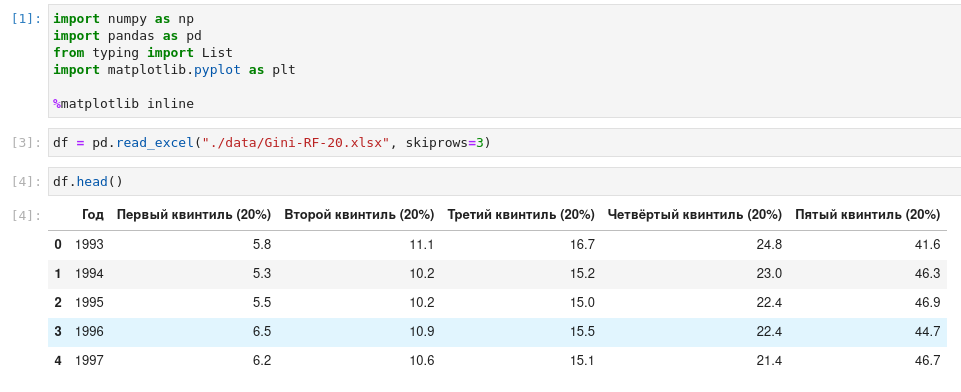
\includegraphics[scale=0.35]{gini1}
	\caption{Данные для квинтилей}
	\label{fig:gini1}
\end{figure}

\newpage

Далее была реализована функция, которая рассчитывает значение коэффициента Джини по входным данным. (Рисунок \ref{fig:gini2})

\begin{figure}[h]
	\centering 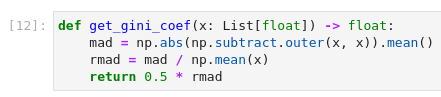
\includegraphics[scale=0.6]{gini2}
	\caption{Функция для расчёта коэффициента Джини}
	\label{fig:gini2}
\end{figure}

После чего, по данным были произведены расчёты. (Рисунок \ref{fig:gini3})

\begin{figure}[h]
	\centering 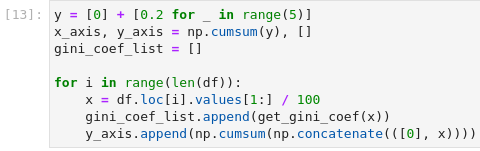
\includegraphics[scale=0.6]{gini3}
	\caption{Расчёт коэффициента Джини}
	\label{fig:gini3}
\end{figure}

Таким образом, на основе коэффициентов Джини была получена визуализация кривой Лоренца. (Рисунок \ref{fig:gini4})

\begin{figure}[h]
	\centering 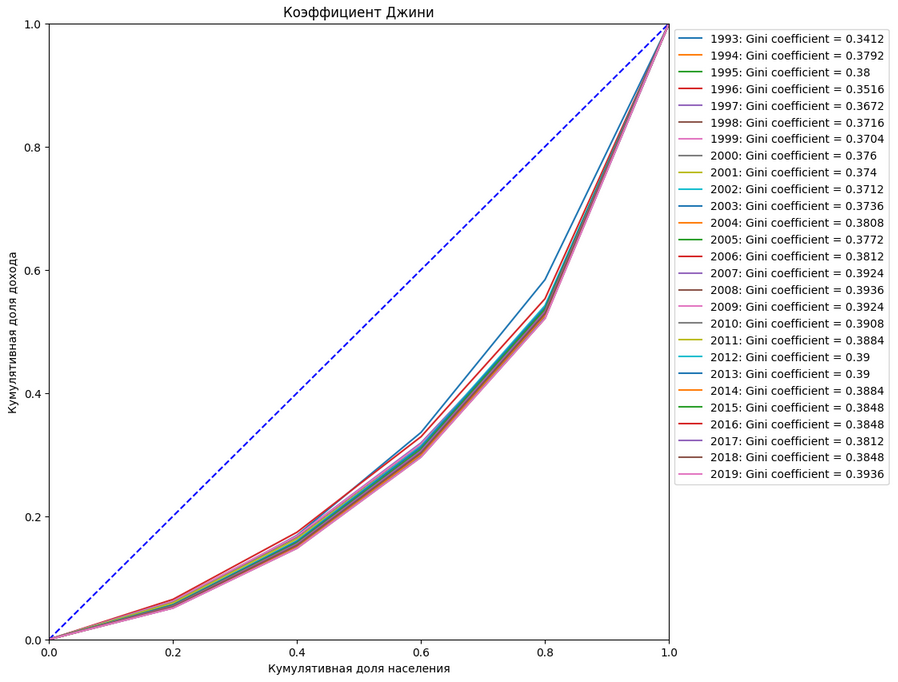
\includegraphics[scale=0.32]{gini4}
	\caption{Кривая Лоренца}
	\label{fig:gini4}
\end{figure}

Таким образом, нами были рассчитаны коэффициенты Джини и построены кривые Лоренца для доли доходов по квинтилям РФ. Исходя из полученных результатов можно сделать вывод о том, что расслоение по доходам в РФ было приемлемым, так как значение коэффициента Джини за все года было меньше значения 0.4.